\documentclass[11pt]{labbook}
\usepackage[utf8]{inputenc}
\usepackage{graphicx}
\usepackage{csquotes}
\usepackage{float}
\usepackage[margin=1in]{geometry}
\usepackage{setspace}
\usepackage{listings}
\usepackage{color}
\usepackage{array}
\usepackage{xspace}
\usepackage{times}
\usepackage{amssymb, amsmath}
\usepackage{fancyhdr}
\usepackage[]{algorithm}
\usepackage[noend]{algpseudocode}
\usepackage{courier}

\newcolumntype{P}[1]{>{\centering\arraybackslash}p{#1}}

\definecolor{dkgreen}{rgb}{0,0.6,0}
\definecolor{gray}{rgb}{0.5,0.5,0.5}
\definecolor{mauve}{rgb}{0.58,0,0.82}


\textwidth=16.5cm %mikeg: June 18, 2016 - Why is this being set?  It should be set by geometry package

\lstset{frame=tb,
  language=Java,
  aboveskip=3mm,
  belowskip=3mm,
  showstringspaces=false,
  columns=flexible,
  basicstyle={\small\ttfamily},
  numbers=none,
  numberstyle=\tiny\color{gray},
  keywordstyle=\color{blue},
  commentstyle=\color{dkgreen},
  stringstyle=\color{mauve},
  breaklines=true,
  breakatwhitespace=true,
  tabsize=3
}


%%%%%%%%%%%%%%% BEGIN LOCAL COMMANDS %%%%%%%%%%%%%%%%%%%
\newcommand{\DeltaEta}{\ensuremath{\Delta\eta}\xspace}
\newcommand{\DeltaM}{\ensuremath{\Delta M}\xspace}

%%%%%%%%%%%%%%% END LOCAL COMMANDS %%%%%%%%%%%%%%%%%%%


%%%%%%%%%%%%%%% BEGIN LOCAL CUSTOMIZATIONS %%%%%%%%%%%%%%%%%%%
\usepackage{etoolbox}
\makeatletter
%suppress pagebreaks between days
\patchcmd{\addchap}{\if@openright\cleardoublepage\else\clearpage\fi}{\par}{}{}
\makeatother 

%%%%%%%%%%%% END LOCAL CUSTOMIZATIONS %%%%%%%%%%%%%%%%%


\title{Notes for Undergraduate Research Work}
\author{Alan Dixon}

\begin{document}

\labday{June 6, 2016 Notes}

\begin{itemize}
    \item Discovered and fixed two bugs involving an uninitialized selection vector and Mphi values
    \item Said bug fixes resolved the issue of the program crashing around iteration 2500
      
    \item Despite the fixed bugs resolving that issue, log likelihood values still plummet to values eventually reaching 10e-23 which causes the not a number error, causing the MCMC algorithm to halt.
\footnote{mikeg: Is this a typo?  Usually it is $\exp{-300}$ that starts to push the limit of numerical precision.
Further, it is unclear to me why this would cause a problem unless you are later converting this number back to a log scale.  
Is it necessary to exponentiate and then take the log?
}
\footnote{mikeg: This is confusing given the previous statement. 
  It sounds like you didn't really resolve the underlying issue.}
    \item Due to Newton failing to execute my job request, I had to run the R script on my laptop so I was only able to run it once so more testing is needed but for the meantime it appears it takes until around iteration 42000 for the program to crash.
      \footnote{why is newton failing to execute your job requests? 
        How and when will you solve this issue?}
    \end{itemize}

TODO:\\
    Work on psuedocode\\
    Remove redundancies\\
    Determine if Sphi prior is being used\\
    Improve varialbe names and documentation\\
    Document the R scripts\\
    
\labday{June 7, 2016}

\begin{itemize}
    \item Removed exit statements from FONSEParameter.cpp, PANSEParameter.cpp, and RFPParameter.cpp in order to eliminate warnings when running the check in R
    \item Downloaded all of the necessary files to my Gauley account.
    \item Running FONSE with simulated data and b = 0.001 led to "nan" being reached much more quickly than on my laptop, around iteration 5500.
      \footnote{mikeg: is this based on one run on each machine?
        It's more useful to be more quantitative and descriptive} 
    \item Said issue may be a cause of R not working correctly on Gauley as compared to my laptop. 
      Multiple errors and missing packages were encountered. 
      These errors made it impossible to check any plots.
\item{mikeg: If it strange you're running into such errors since gauley is used to develop the code base.
    Are they really errors or, since you execute code, warnings?
    What are the error codes?  
    When discussing errors, it is good to always include some output using the 'quote' or similar environment in \LaTeX.
    Do other people run into these same errors?
  }
    \item Two new Items for the TODO list: Continue troubleshooting R on Gauley and alter Jeremy's .sge scripts so that they no longer email him when I run a job on Newton.
\end{itemize}

\labday{}{June 8, 2016}

\begin{itemize}
    \item Changed the .sge scripts for Newton so that Jeremy no longer receives an email upon the completion of a job.
    \item Changed a function in FONSEModel.cpp to match it's corresponding function in ROCModel.cpp. In particular, I changed a long series of divisions to on division and a series of multiplications because multiplication is a faster operation.
      \footnote{mikeg: include the function name. 
        Any information on speed up?
      }
    \item Fixed a typo in the documentation of ROCModel.cpp
    \item Worked out some kink experienced while running R scripts on Gauley. In particular, finally made it so that the plots actually showed up and worked. 
    \item Formulated the hypothesis that the reason we are experiencing a drop in log likelihood comes from a bug involving either deltaM, deltaOmega, or phi after observing the trace plots.
\footnote{Include plots in your notes, especially if you refer to them, and explain more clearly why you think its behavior indicates this.
}
\end{itemize}


\labday{June 13, 2016}

\begin{itemize}
    \item Fixed an error in FONSEModel.cpp involving a couple of missing semicolons
    \item Fixed an error in the .tex file for the notes where using the hyperref package kept the notes from compiling
    \item After running FONSE again, with simulated data and b = 0.001, it seems the errors in log likelihood are no longer deterministic. Values still plummet, and the traces suggest that both mutation and selection values may be the cause. Further testing and observation is required.
      \footnote{mikeg: June 16, 2016 - If you run the code in serial and set the random number seed, does the behavior become repeatable?}
    \item Found a difference between FONSEModel and ROCModel where ROC would take mutation prior into account and FONSE wouldn't. This might part of the issues causing log likelihood values to plummet, but testing is required.
    \item Uploaded both the new .tex file and its corresponding pdf just in case there's another error that doesn't keep me from compiling on my machine but might keep another from compiling on a different machine.
      \footnote{mikeg: June 16, 2016 - In general, you should refrain from making copies of files (e.g.~labNotes  $\rightarrow$ Lab\_Notes). 
        Instead, rely on the fact that you are using version control and can always revert back or merge with an earlier version of a file.
     }
\end{itemize}

\labday{June 14, 2016}

\begin{itemize}
    \item The addition of the mutation prior into FONSE seems to have stopped the rapid descent of the Log Likelihood values. After running it once with 1000 samples and 1 thining, the log likelihood stayed somewhat stable after starting low and rising to about -20000. The vaules were also similar when running with 1000 samples and 10 thining. More extensive testing is required to ensure that the plummeting problem is finally resolved.
      \footnote{mikeg: June 16, 2016 -
        I am glad that the prior seems to have fixed this problem.  
        I don't understand, however, why it did so.  
        Were the \DeltaM values diverging from the true value substantially?
        Note also that one can relax the effect of the prior by making its $\sigma_\DeltaM$ value large. 
        In fact at the $\lim_{\sigma_\DeltaM \rightarrow \infty}$ the system essentially behaves as if it has a flat prior (which is proportional to 'no prior').
}
        
    \item Although the log likelihood values are starting to come together, there is an issue observed in both the mutation and selection traces where certain codons are not being accepted. 
    \item Conducted further comparisons on FONSE and ROC to remove redundancies and semantic oversight.
\end{itemize}

\labday{June 15, 2016}

\begin{itemize}
    \item After running FONSE overnight, I feel it's safe to conclude that the plummeting log likelihood problem is resolved although there have been issues with multiple, sometimes all but a few, codons with acceptance rates of 0 as backed up by both the output and the trace plots of both mutation and selection, although this is again non deterministic. Running it on Gauley produced far more codons with no impact than when I ran it on my laptop so the non determinism may come from memory or operating system differences.
\footnote{mikeg: June 16, 2016 -
  This shouldn't happen since we are using an MCMC whose step sizes adapt based on the acceptance ratio of the previous samples. 
  (Of course, it would be good to make sure this adaptive option is set.)
  We saw similar 'non-acceptance' behavior with Gabe and/or Jeremy in the past month or two.
  It had to deal with the parameters not being correctly referenced or defined.
  Cedric will remember the details.
}
    \item There was a problem with Gauley involving the machine randomly restarting without being prompted. It doesn't seem like a major problem and the effects seem to be confined to the processes being run on it at the time being prematurely terminated. I'll be keeping an eye for any unespected behavior from Gauley in case the problem ends up being reoccuring.
    \item Studied the model to try and deduce how the simple inclusion of the mutation priors resolved the plummeting problem. So far it still remains fairly unclear and more studying is necessary. 
\end{itemize}

\labday{June 16, 2016}
    \begin{itemize}
        \item Ran FONSE with b = 0.001, samples = 1000, and Thinning = 10 3 separate times. \footnote{mikeg: June 18, 2016- Where all three of these runs carried out with the same set of genes?
If not, then LLik(data$\|$parmeters) surfaces, although similiar, will differ between the runs.
'}
        \item Run 1 \footnote{mikeg: June 18, 2016 - Per my previous request, please include the relevant figures.
        I recommend organizing figures by putting them in a separate folders such as ``Figures/2016/June/16''.
        You should also name them in a consistent manner such as ``FONSE\_run\_1\_trace\_LLik.png''
      }
        \begin{itemize}
          \item Log likelihood settled around -9600
          \item AA's L and R had acceptance rates of 0
          \item stdDevSynthesisRate posterior estimate settled around 1.4, .05 for the proposal width
          \item Trace of the expected values of phi goes to 0.
          \item All codons for L in the mutation traces stop changing and fall out around sample 100 \footnote{mikeg: June 18, 2016 - what does 'fall out' mean?}
          \item R falls out around sample 300
          \item It's the same story for both L and R in the selection traces except it takes about half as many samples for both to fall out
        \end{itemize}
        \item Run 2 \footnote{mikeg: June 18, 2016 - again, figures should be included to help illustrate and document the behavior you describe.}
        \begin{itemize}
            \item Log likelihood settled around -14000
            \item AA's L and R still had acceptance rates of 0 \footnote{mikeg: June 18, 2016 - Have you described this behavior to Cedric? 
                We've seen similar behavior before.}
            \item stdDevSynthesisRate posterior estimate settles around 1.9, .045 for the proposal width
            \item Trace of the log likelihood didn't level off as much. It seemed to still be rising. 
            \item expected phi trace was the same as Run 1
            \item L falls out around the same place in Mutation as Run 1; R falls out twice as fast.
            \item Both fall out twice as fast in the selection traces compared to Run 1.
        \end{itemize}
        \item Run 3
        \begin{itemize}
            \item Log likelihood settled around -20000
            \item AA's L and R still had acceptance rates of 0
            \item stdDevSynthesisRate posterior estimate settled around 2.5, .04 for the proposal width
            \item There was a more pronounced level-off in the log likelihood trace, much like Run 1
            \item expected phi trace leveled off but slightly above 0
            \item Both L and R had mutation and selection traces similar to Run 1
        \end{itemize}
        \item Also worked on documenting FONSE by taking documentation from similar parts in ROC and making the necessary alterations before putting it into FONSE
         
        \begin{figure}
            \centering
            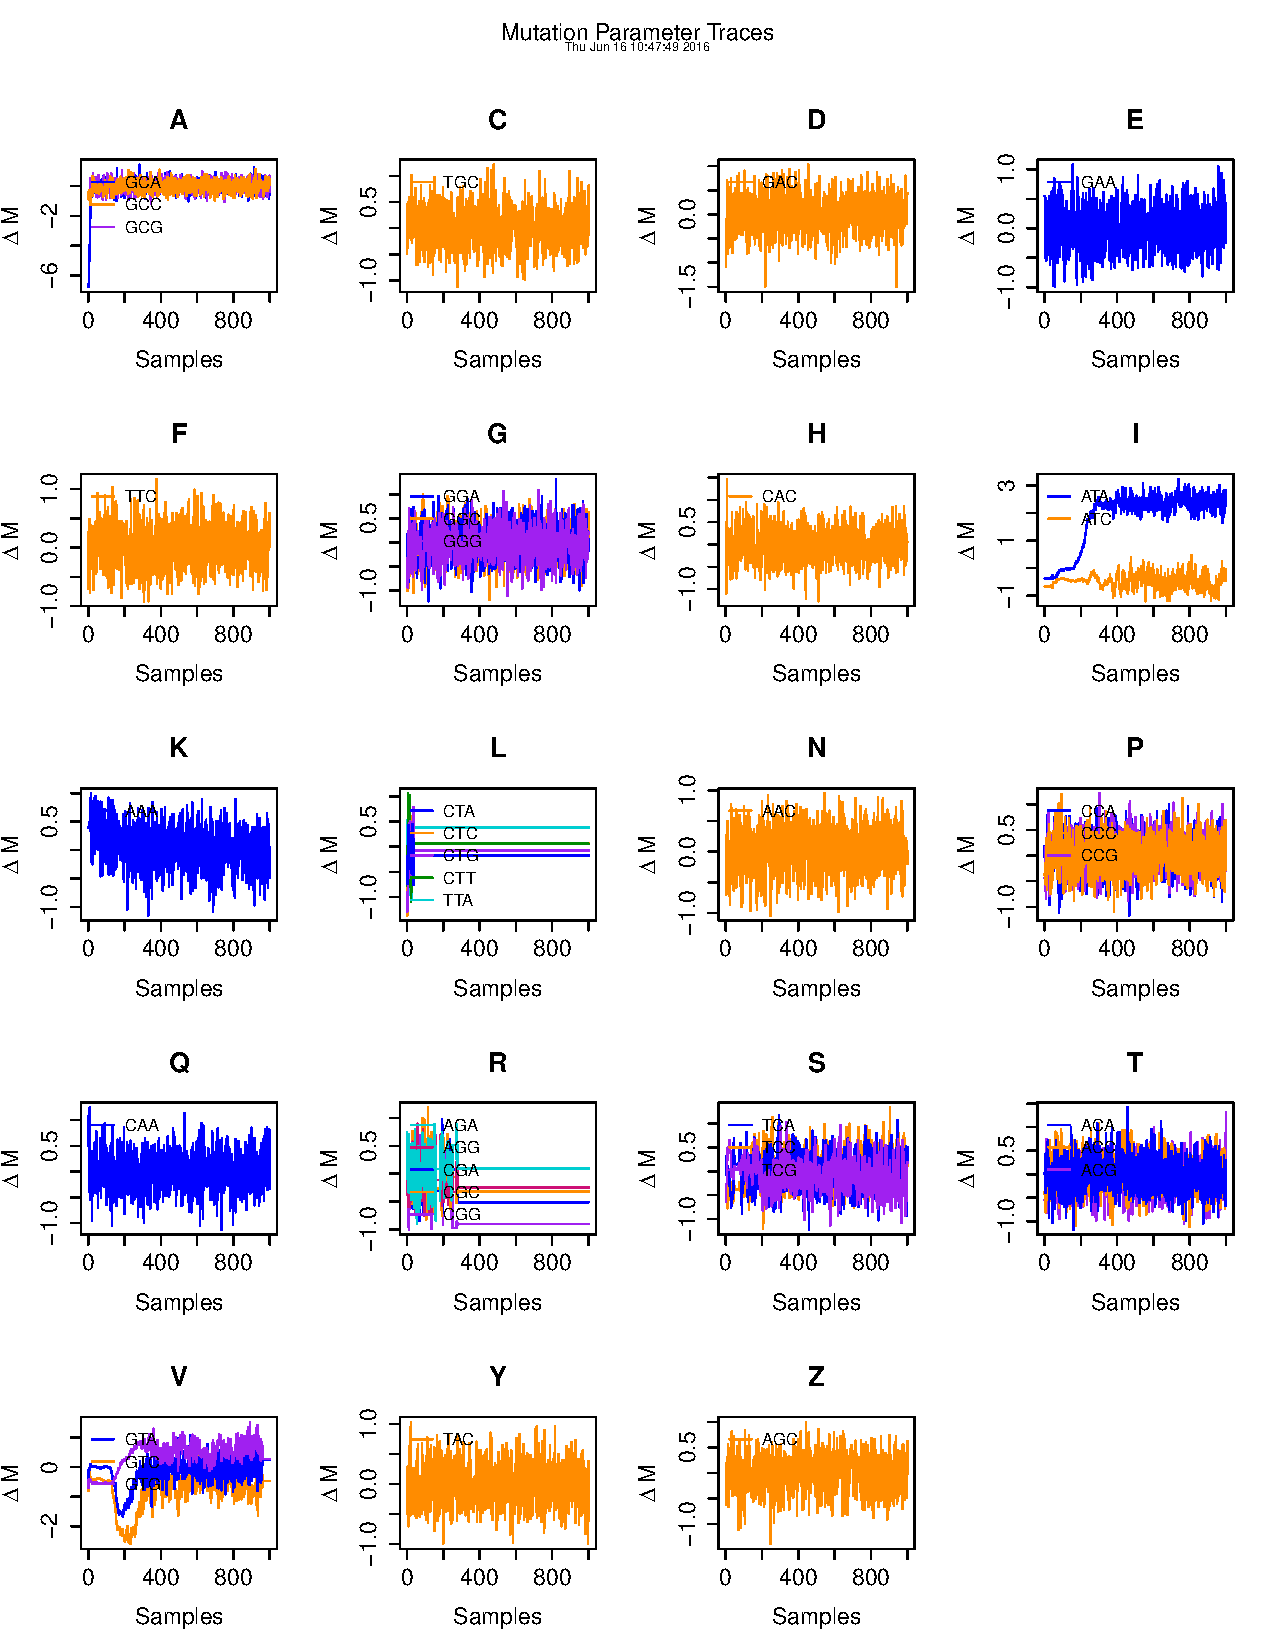
\includegraphics[scale=.65]{FONSE_Plots/June_16/Run1_MutationTrace}
            \caption{Mutation Trace for Run 1}
            \label{fig:JUN16_MUT_R1}
        \end{figure}
        \begin{figure}
            \centering
            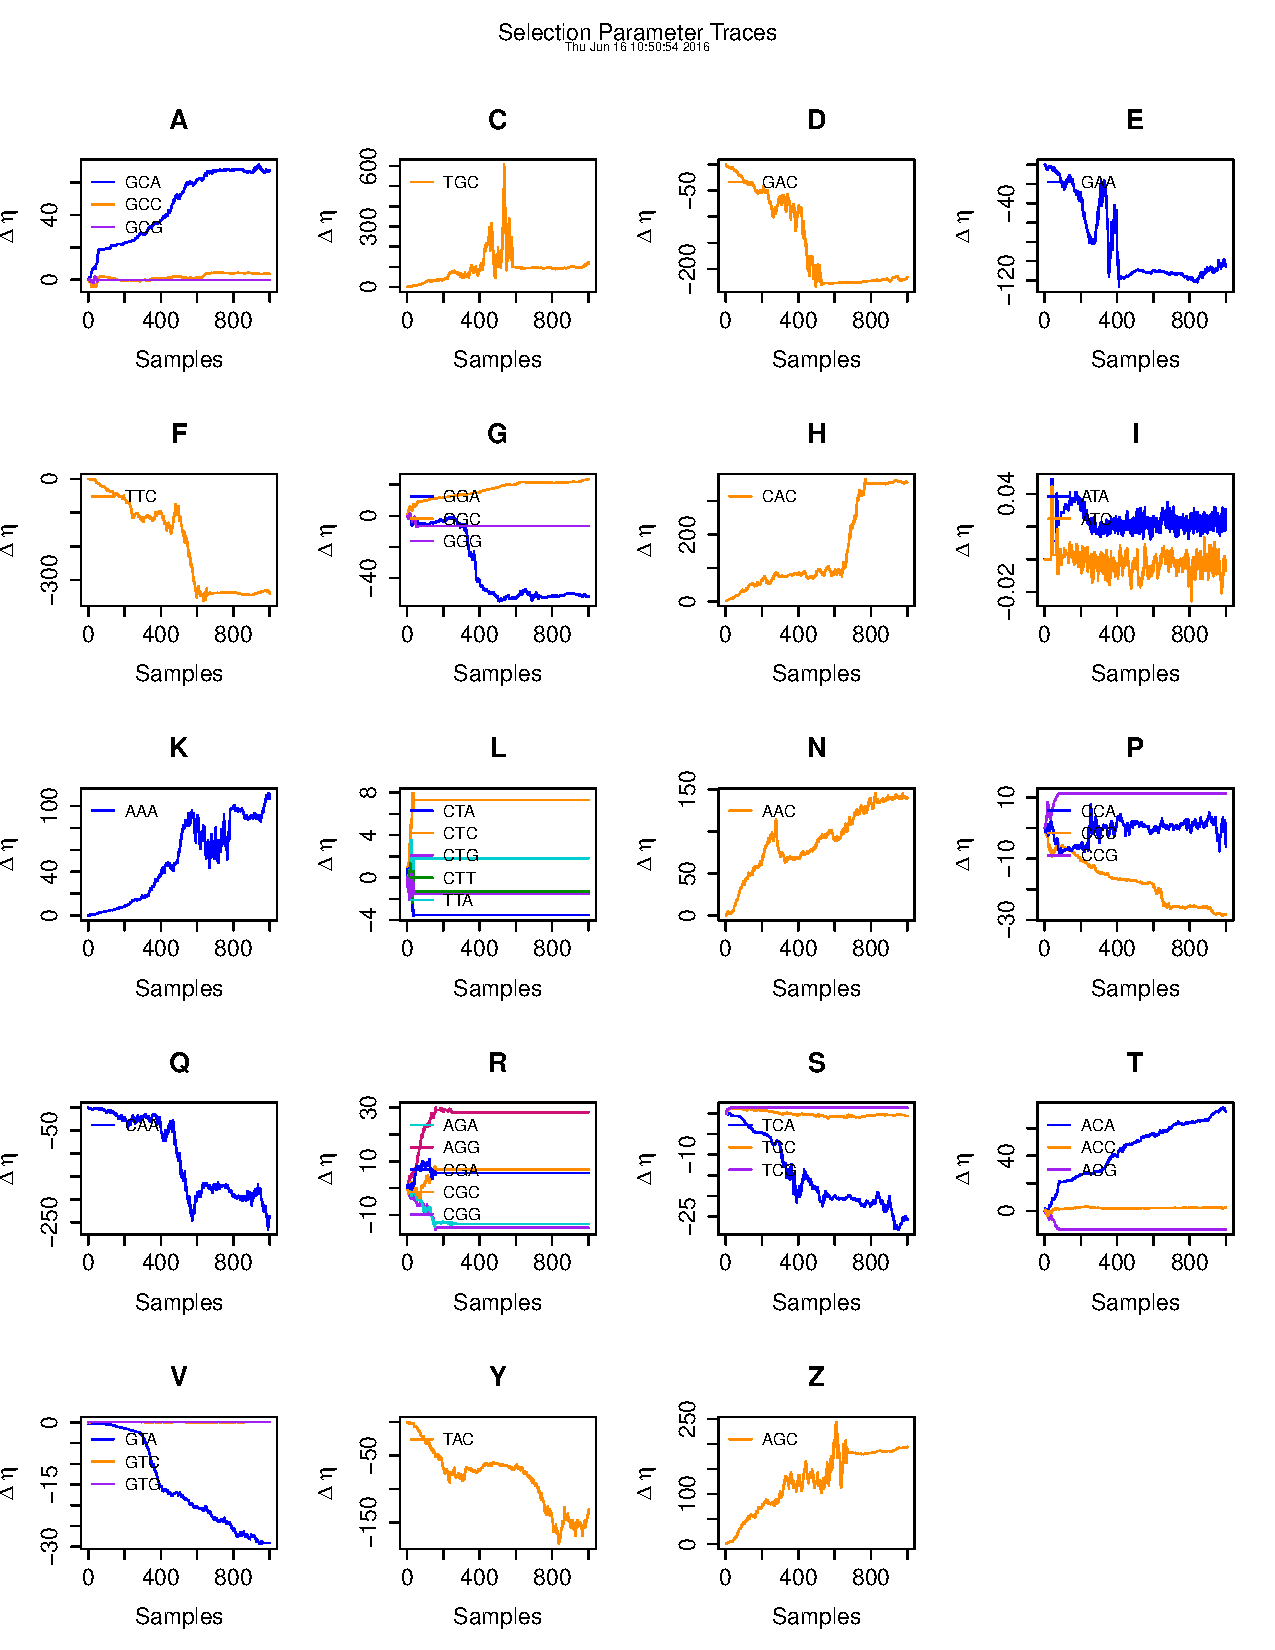
\includegraphics[scale=.65]{FONSE_Plots/June_16/Run1_SelectionTrace}
            \caption{Selection Trace for Run 1}
            \label{fig:JUN16_SEL_R1}
        \end{figure}
        \begin{figure}
            \centering
            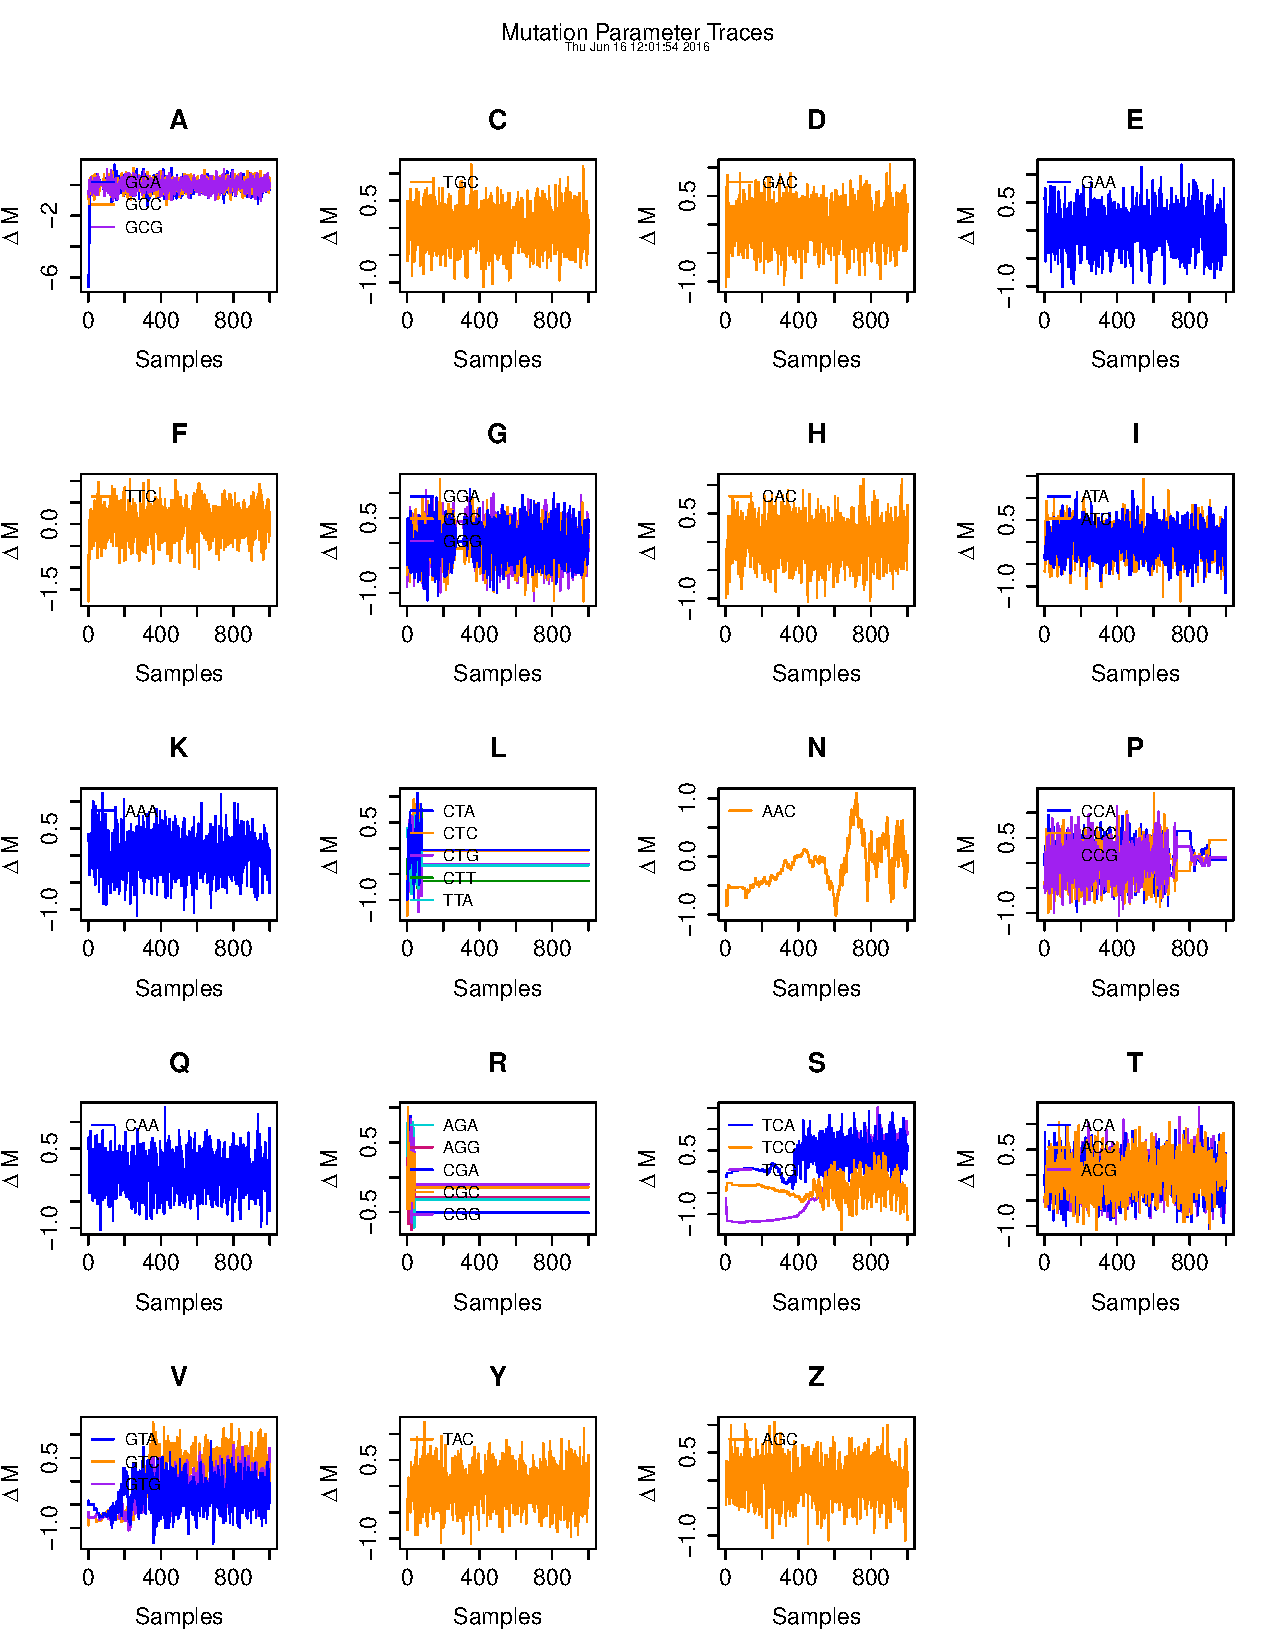
\includegraphics[scale=.65]{FONSE_Plots/June_16/Run2_MutationTrace}
            \caption{Mutation Trace for Run 2}
            \label{fig:JUN16_MUT_R2}
        \end{figure}
         \begin{figure}
            \centering
            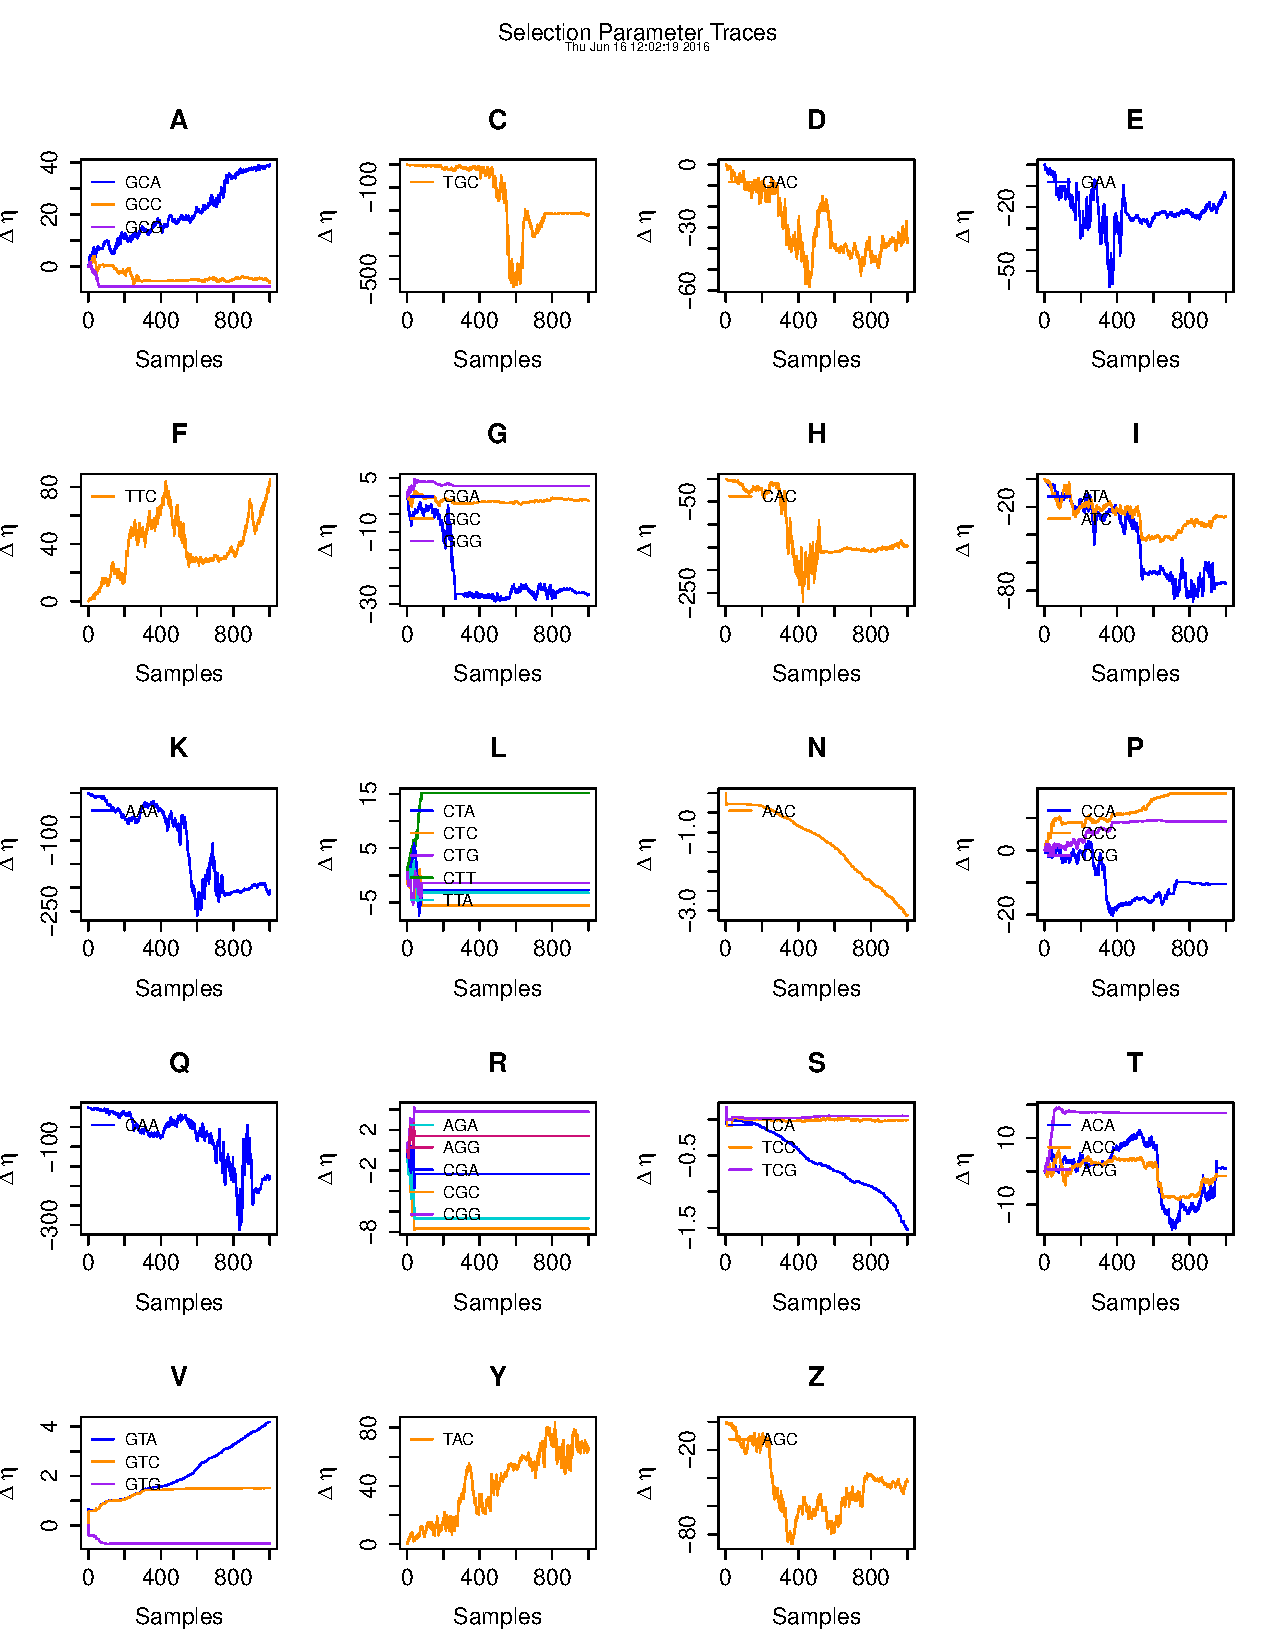
\includegraphics[scale=.65]{FONSE_Plots/June_16/Run2_SelectionTrace}
            \caption{Selection Trace for Run 2}
            \label{fig:JUN16_SEL_R2}
        \end{figure}
        \begin{figure}
            \centering
            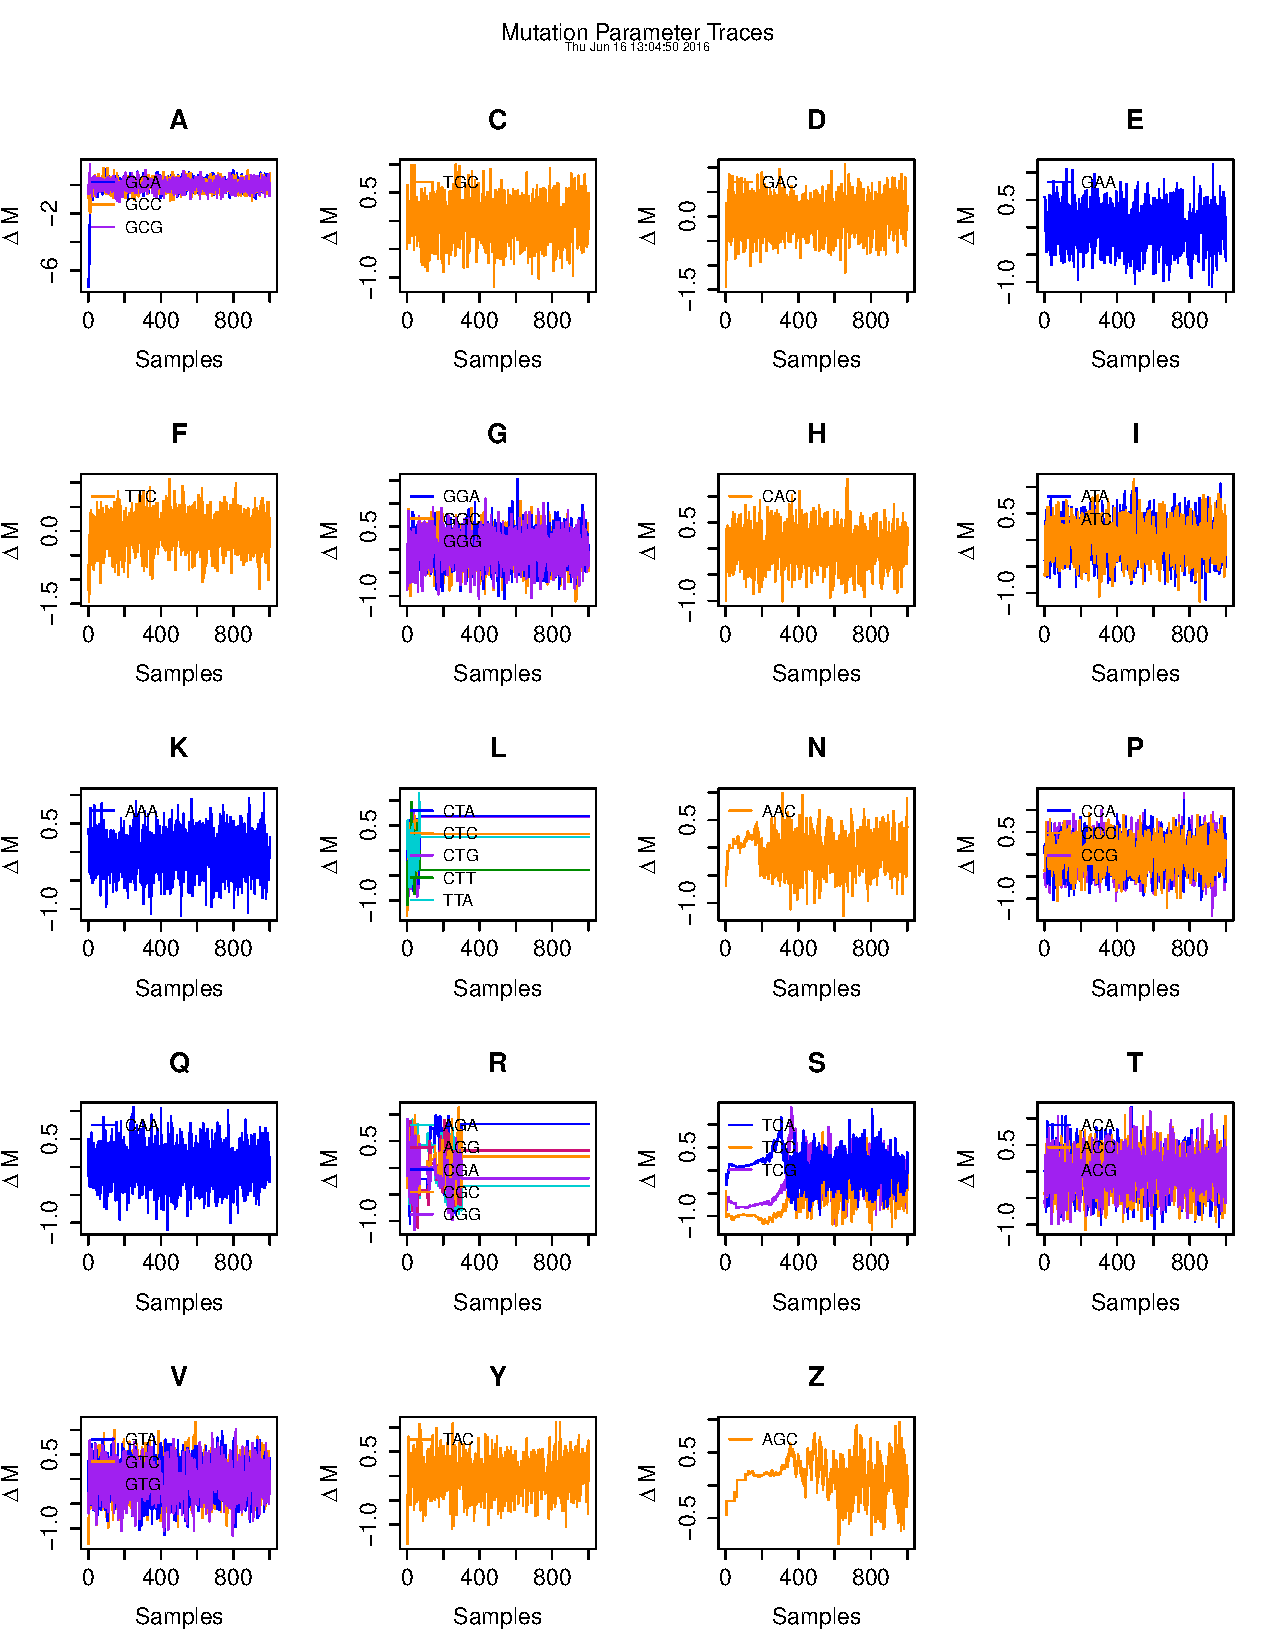
\includegraphics[scale=.65]{FONSE_Plots/June_16/Run3_MutationTrace}
            \caption{Mutation Trace for Run 3}
            \label{fig:JUN16_MUT_R3}
        \end{figure}
        \begin{figure}
            \centering
            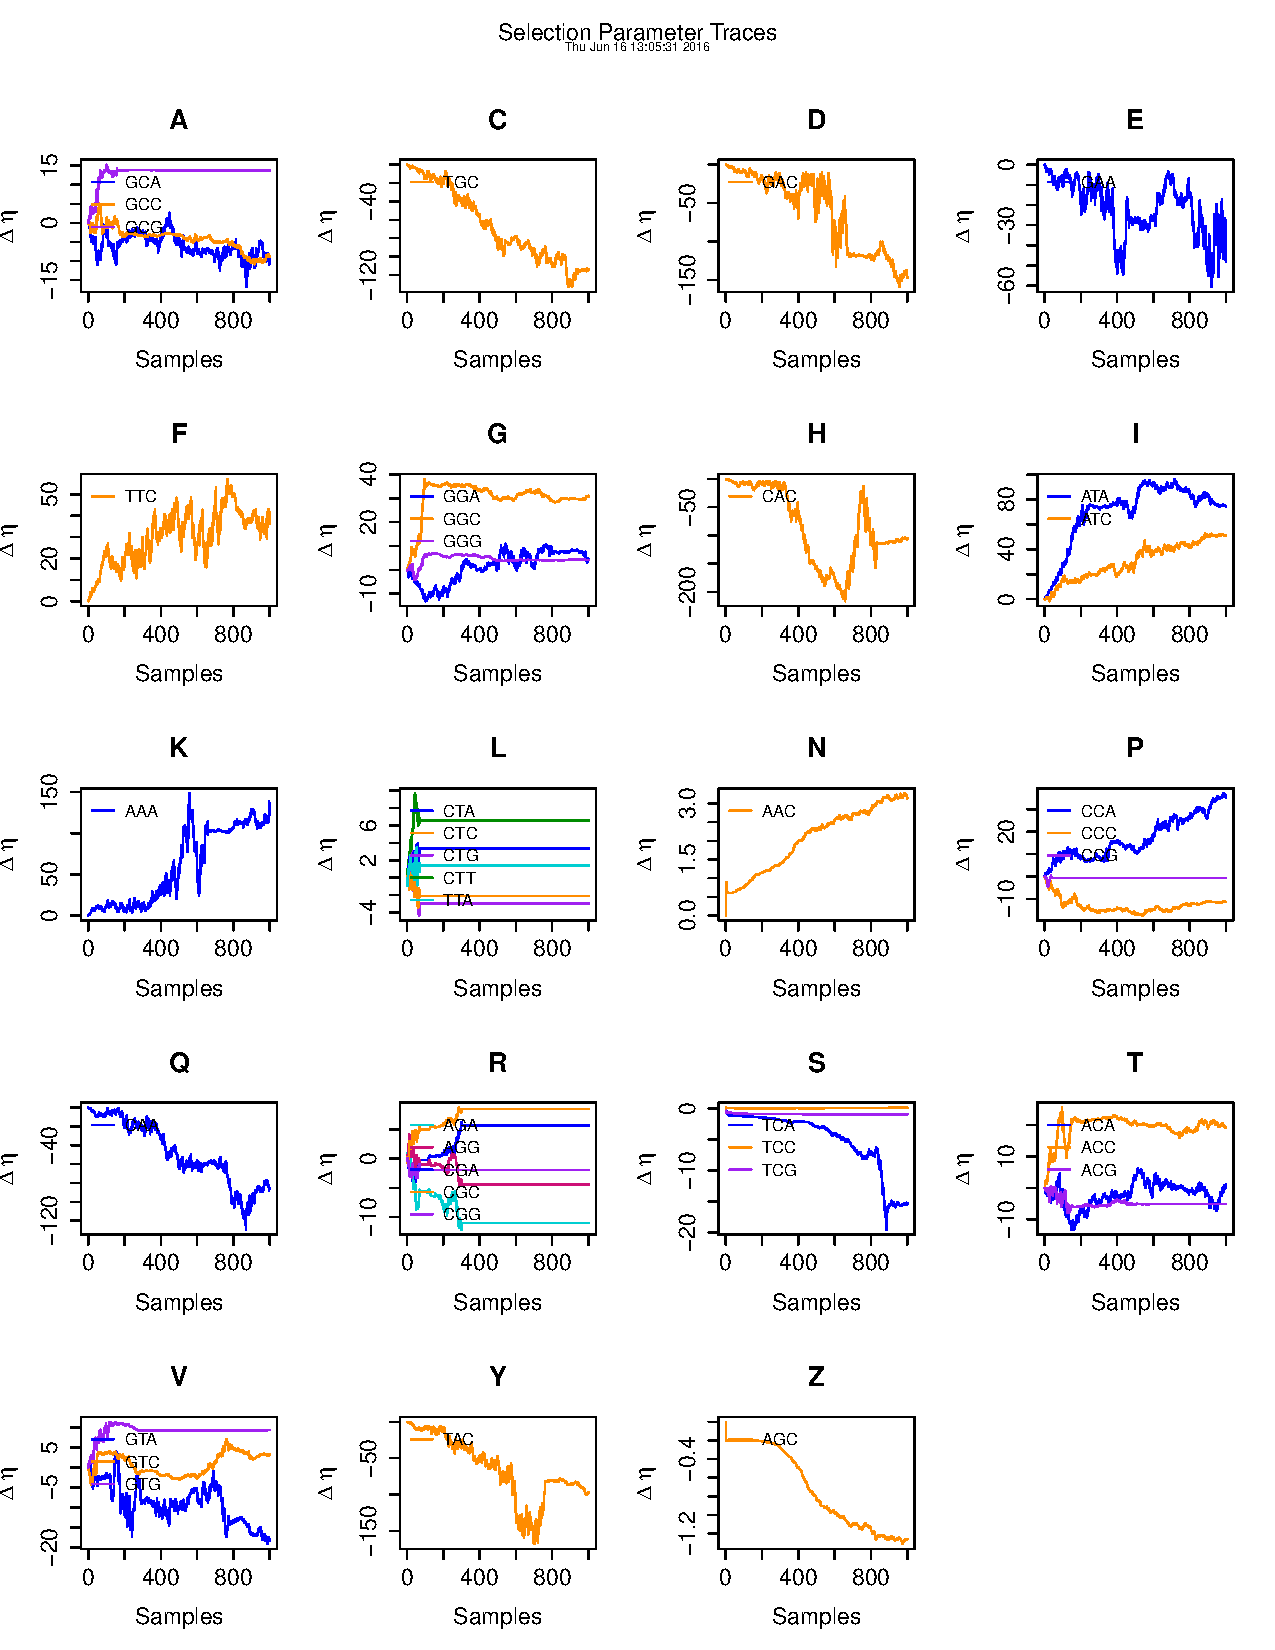
\includegraphics[scale=.65]{FONSE_Plots/June_16/Run3_SelectionTrace}
            \caption{Selection Trace for Run 3}
            \label{fig:JUN16_SEL_R3}
        \end{figure}
    \end{itemize}
    
\labday{June 21, 2016}
    \begin{itemize}
        \item Most of today was spent resolving a problem with RStudio crashing. Both Cedric and I were experiencing this problem so we troubleshooted the issue and discovered that the issue was in a change that had been made in the R-only section of the code in Parameter.cpp. The issue was a "+1" had been added while referencing an element of an array, causing the program to attempt to reference out of the bounds of the array causing a segmentation fault. 
    \end{itemize}
\labday{June 22, 2016}
    \begin{itemize}
        \item Added documentation to the FONSE R-scripts from home due to illness.
    \end{itemize}
    
\labday{June 23, 2016}
    \begin{itemize}
        \item TODO: 
        \begin{itemize}
            \item Alter the code so that there is flexibility when someone invokes a prior i.e. specify whether or not a prior should be used.
            \item run the program with a uniform prior since it is proportional to no prior.
            \item Change from using a covariance matrix to the diagonal to see how that changes the issue where codons have acceptance rates of 0.
            \item Alternatively update the covariance matrix instead.
            \item Check to see if taking the mutation prior out of ROC causes the same phenomenon.
            \item Dump out the values of the genome step of MCMC so we can observe the traces per amino acid.
            \item Put in traces from when the code crashes into the lab notes.
        \end{itemize}
    \end{itemize}
    
\labday{June 24, 2016}
    \begin{itemize}
        \item As requested, I removed the prior from FONSE and ran the model twice in order to get more data and plots showing what's going wrong with the algorithm.
        \item Run 1: b = 0.001, samples = 1000, thinning = 1.
        \begin{itemize}
            \item Log Likelihood values plummet once again. At the end of the MCMC loop the value had reached -1.8e-40. See Figure 7.
            \item Acceptance rates for most of the codons were highly suspect with most having acceptance rates of 1 and others having rates of 0.
            \item Both mutation and selection traces seem consistent with the behavior of the other plots and parameters. See Figures 8 and 9.
        \end{itemize}
        \item Run 2: b = 0.001, samples = 1000, thinning = 10.
        \begin{itemize}
            \item Log Likelihood values plummet once again. At the end of the MCMC loop the value had reached -7.1e-41. See Figure 10.
            \item Acceptance rates for most of the codons were agian highly suspect with most having acceptance rates of 1 and others having rates of 0.
            \item Both mutation and selection traces again seem consistent with the behavior of the other plots and parameters. See Figures 11 and 12.
        \end{itemize}
    \end{itemize}
    
    \begin{figure}
        \centering
        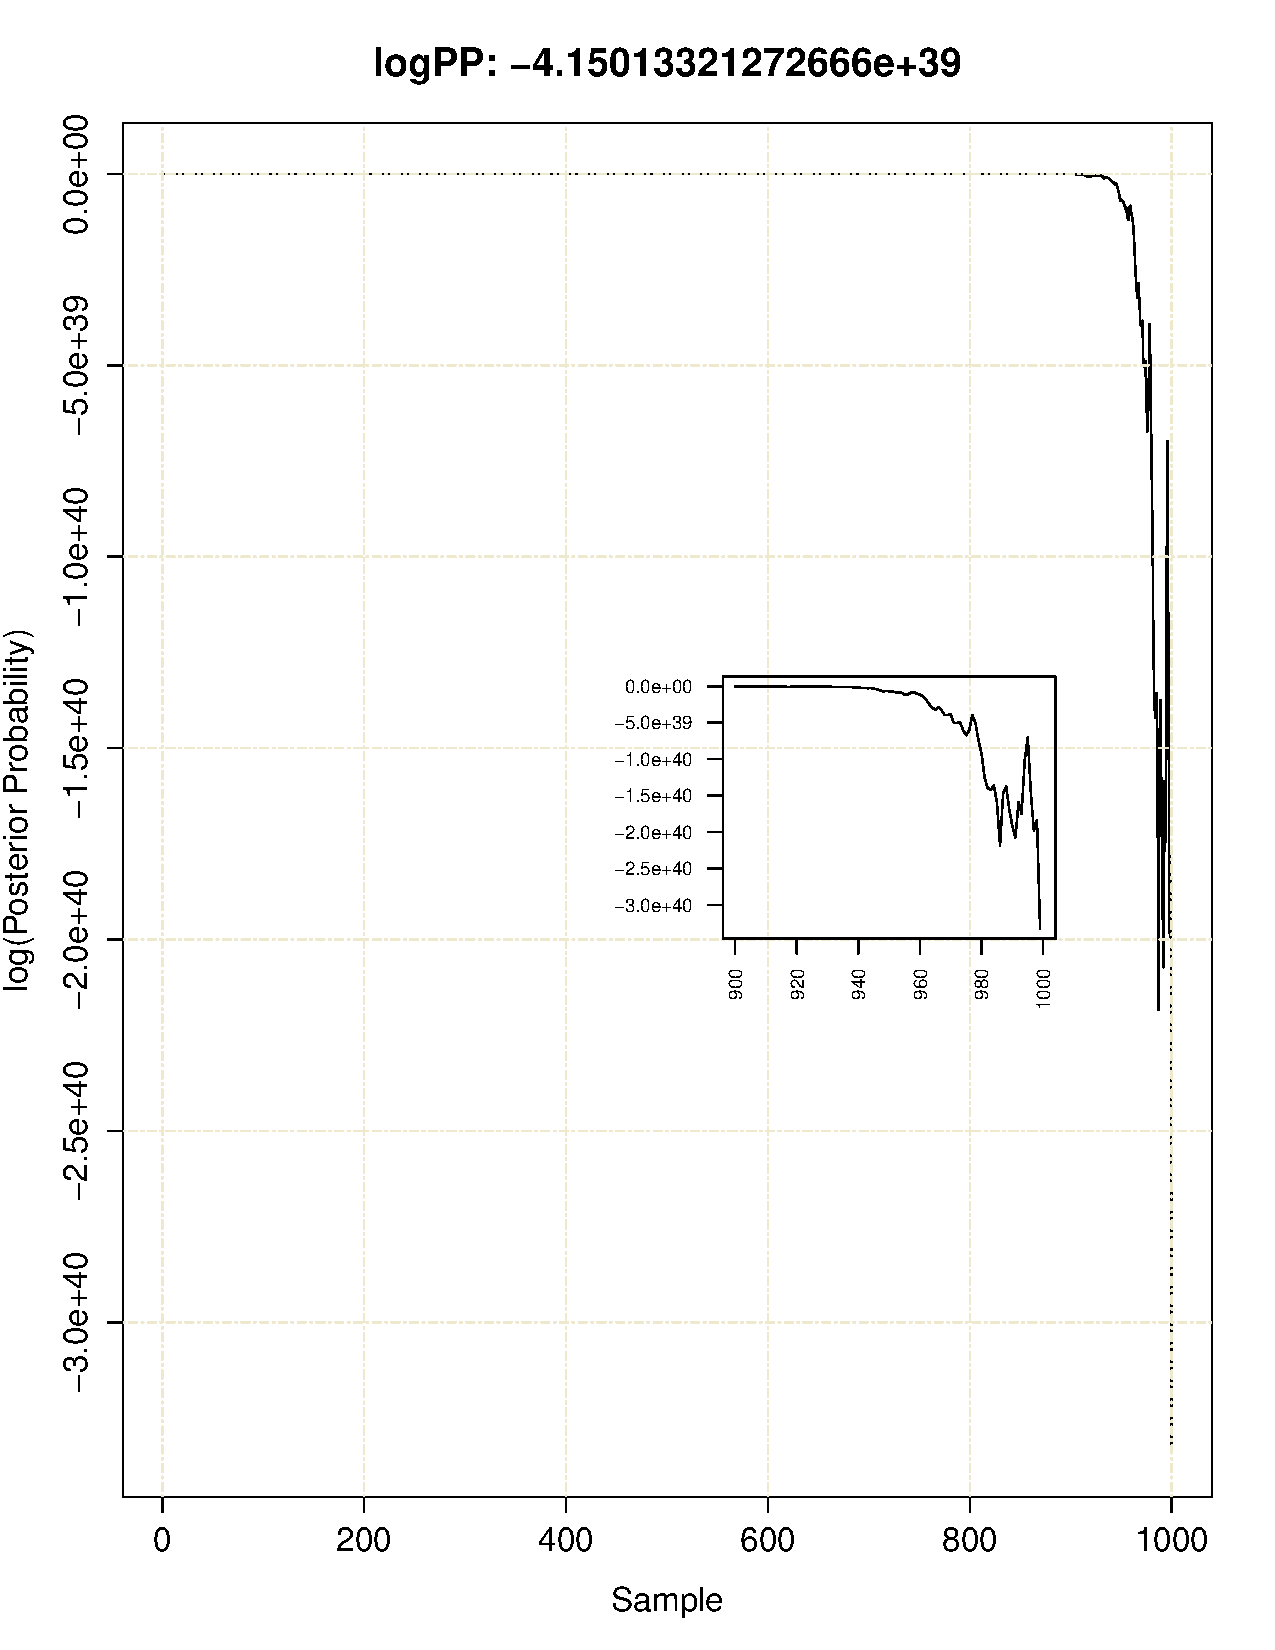
\includegraphics[scale=.65]{FONSE_Plots/June_24/Run1_LogLikeTrace}
        \caption{LogLikelihood trace for Run 1}
        \label{fig:JUN24_LOG_R1}
    \end{figure}
    \begin{figure}
        \centering
        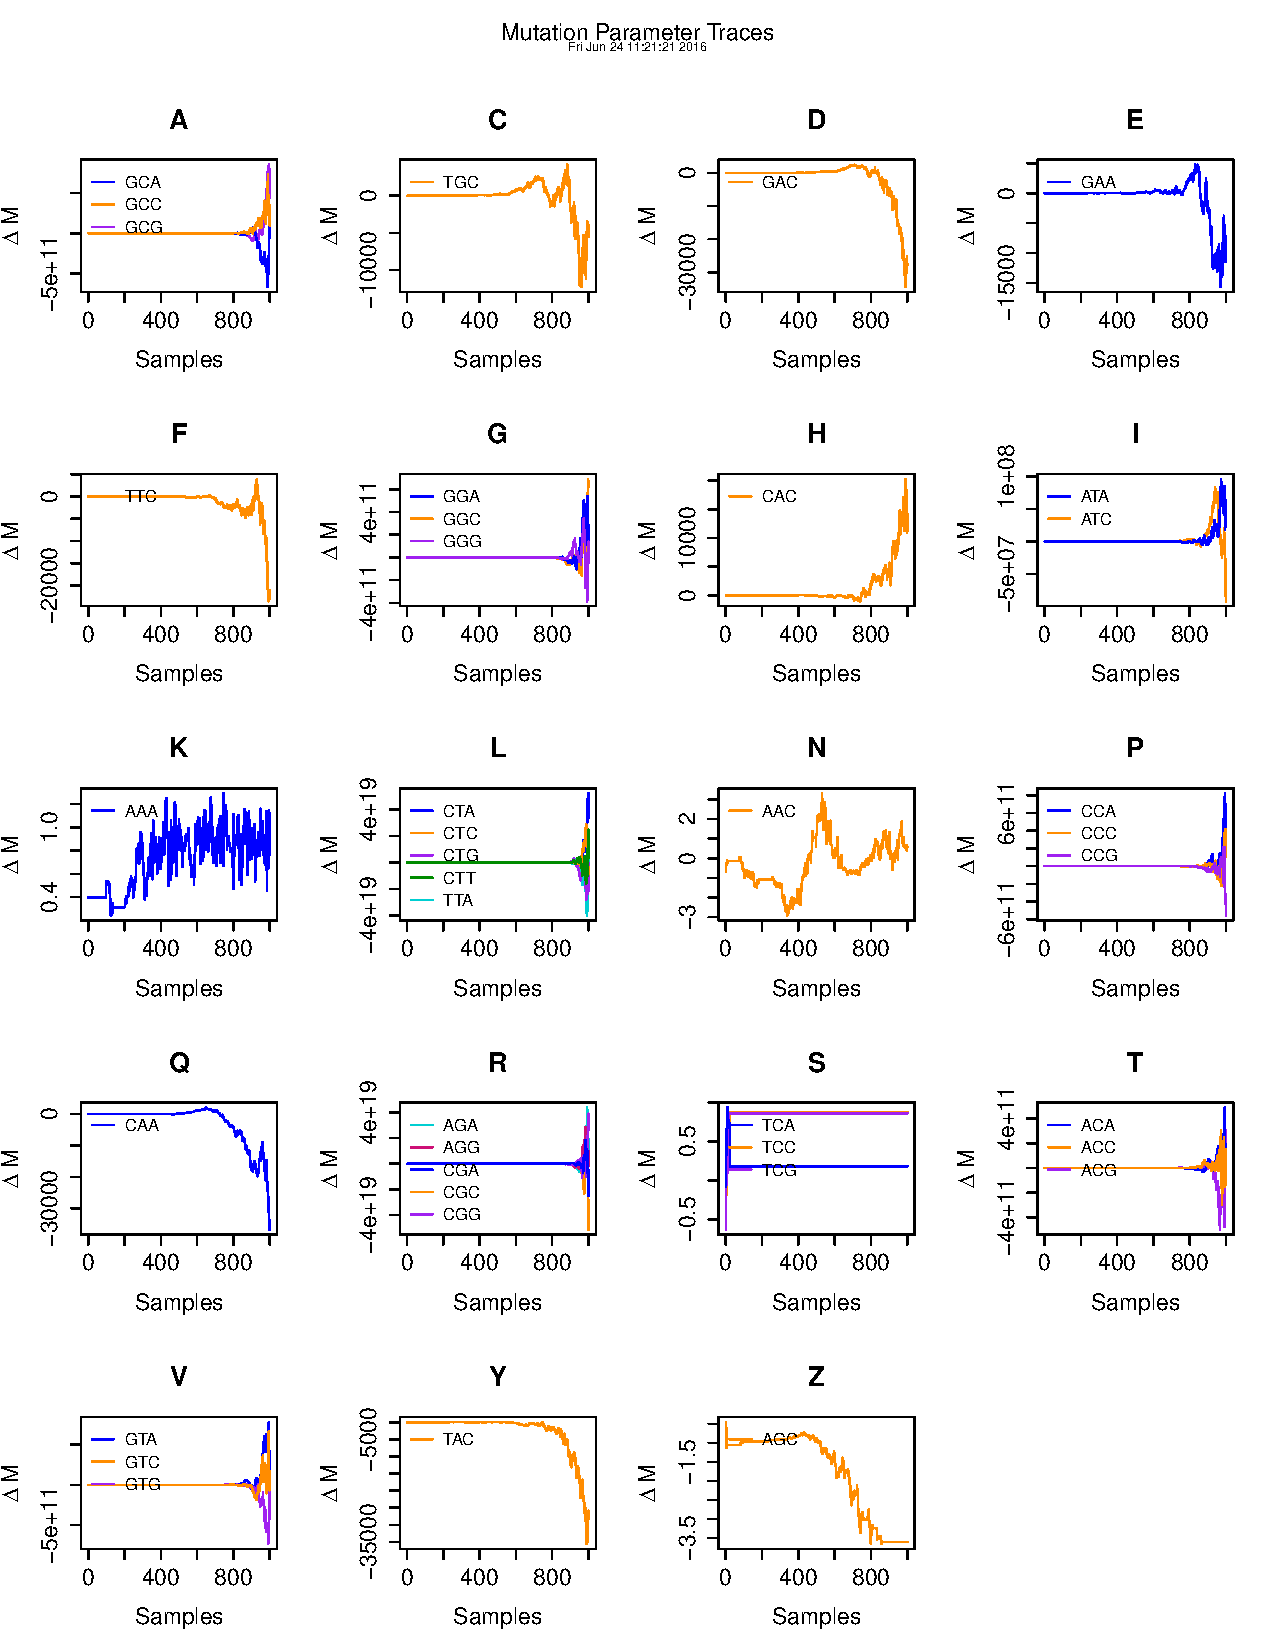
\includegraphics[scale=.65]{FONSE_Plots/June_24/Run1_MutationTrace}
        \caption{Mutation trace for Run 1}
        \label{fig:JUN24_MUT_R1}
    \end{figure}
    \begin{figure}
        \centering
        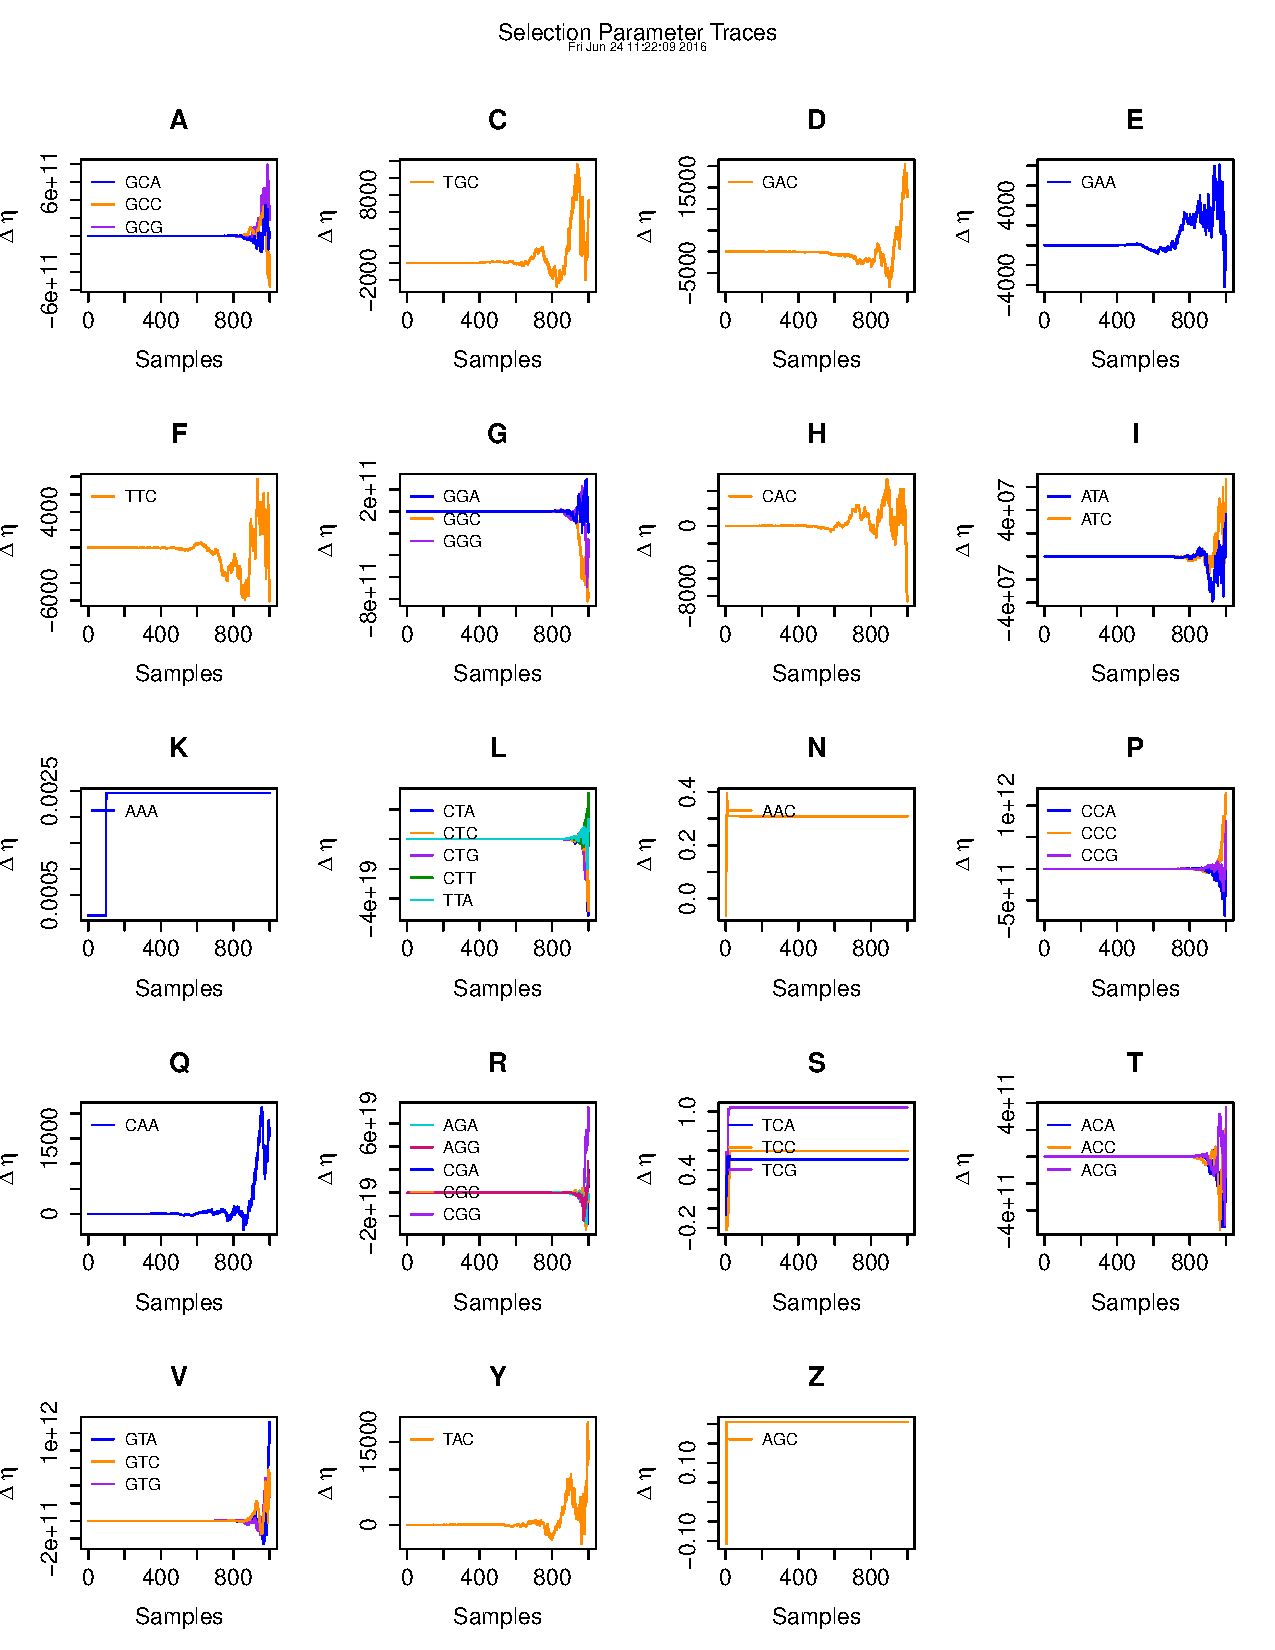
\includegraphics[scale=.65]{FONSE_Plots/June_24/Run1_SelectionTrace}
        \caption{Selection trace for Run 1}
        \label{fig:JUN24_SEL_R1}
    \end{figure}
    \begin{figure}
        \centering
        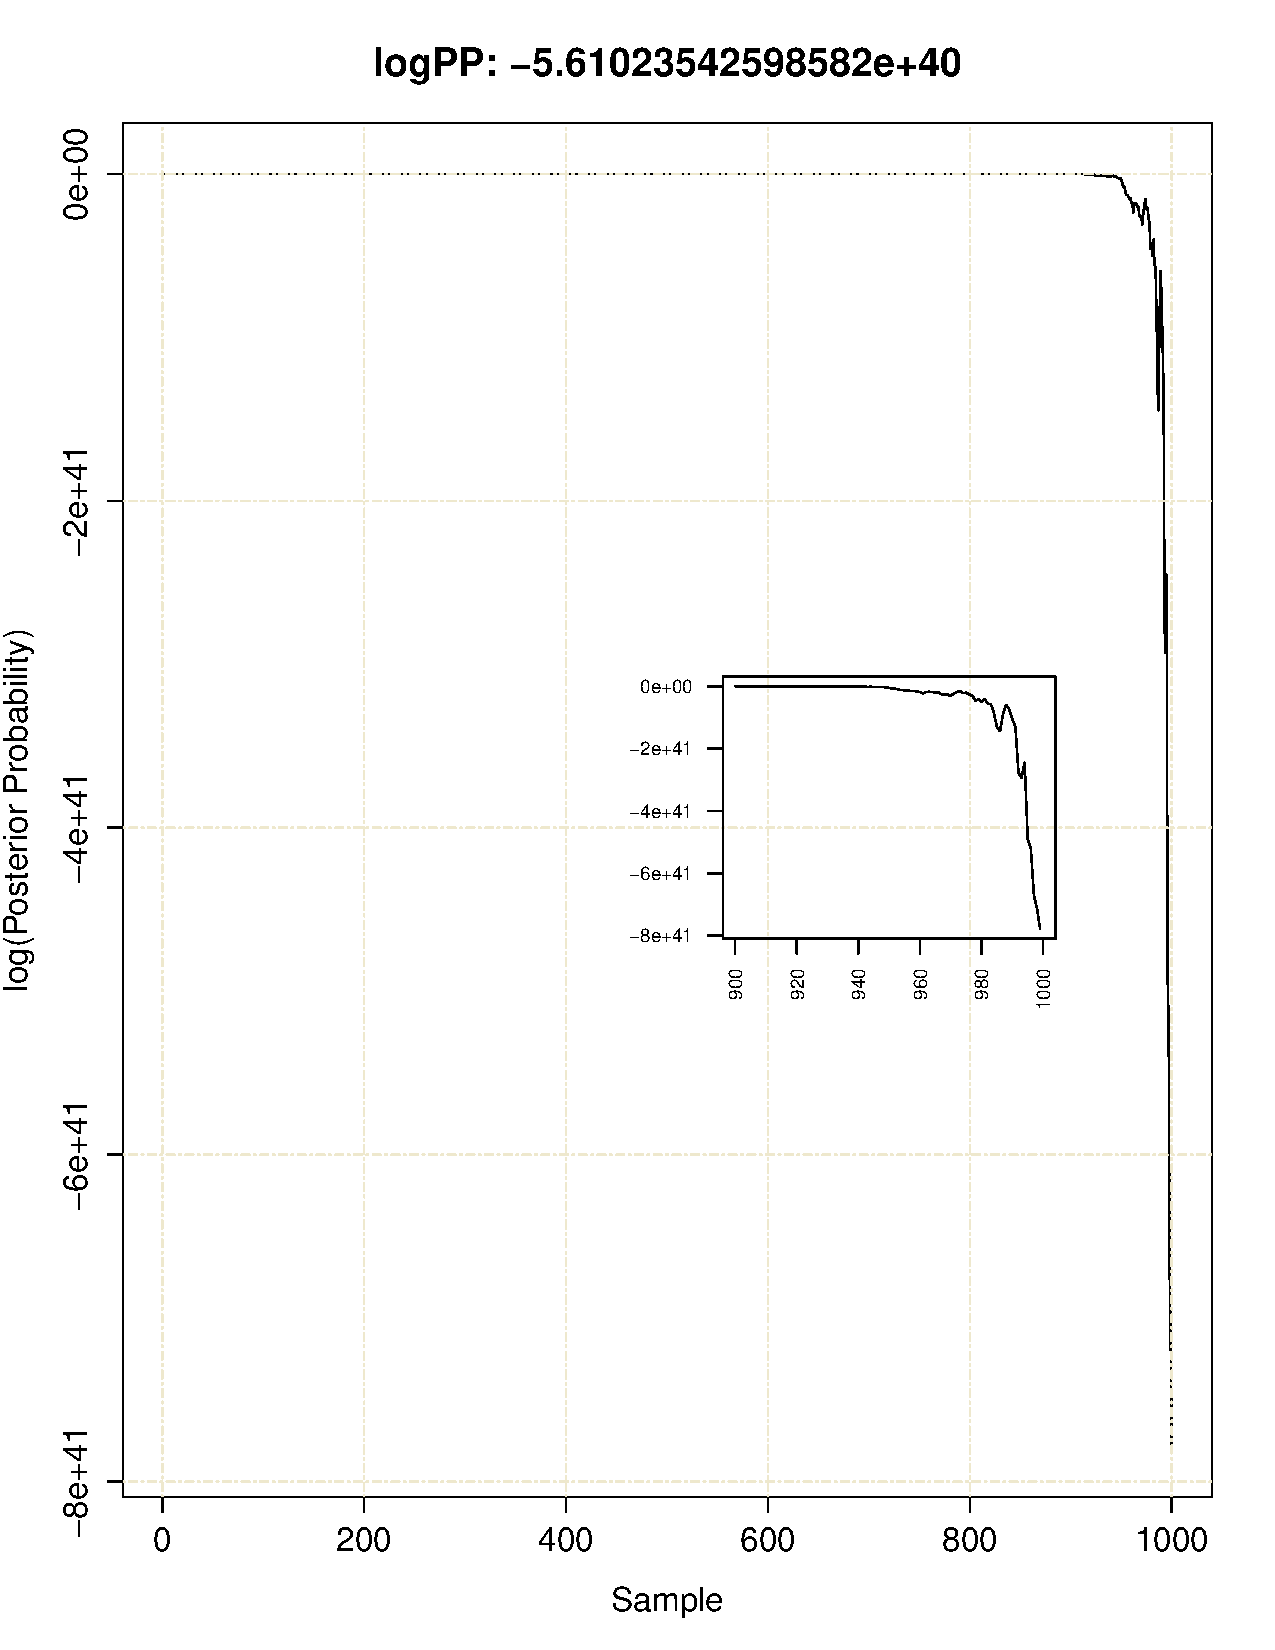
\includegraphics[scale=.65]{FONSE_Plots/June_24/Run2_LogLikeTrace}
        \caption{LogLikelihood trace for Run 2}
        \label{fig:JUN24_LOG_R2}
    \end{figure}
    \begin{figure}
        \centering
        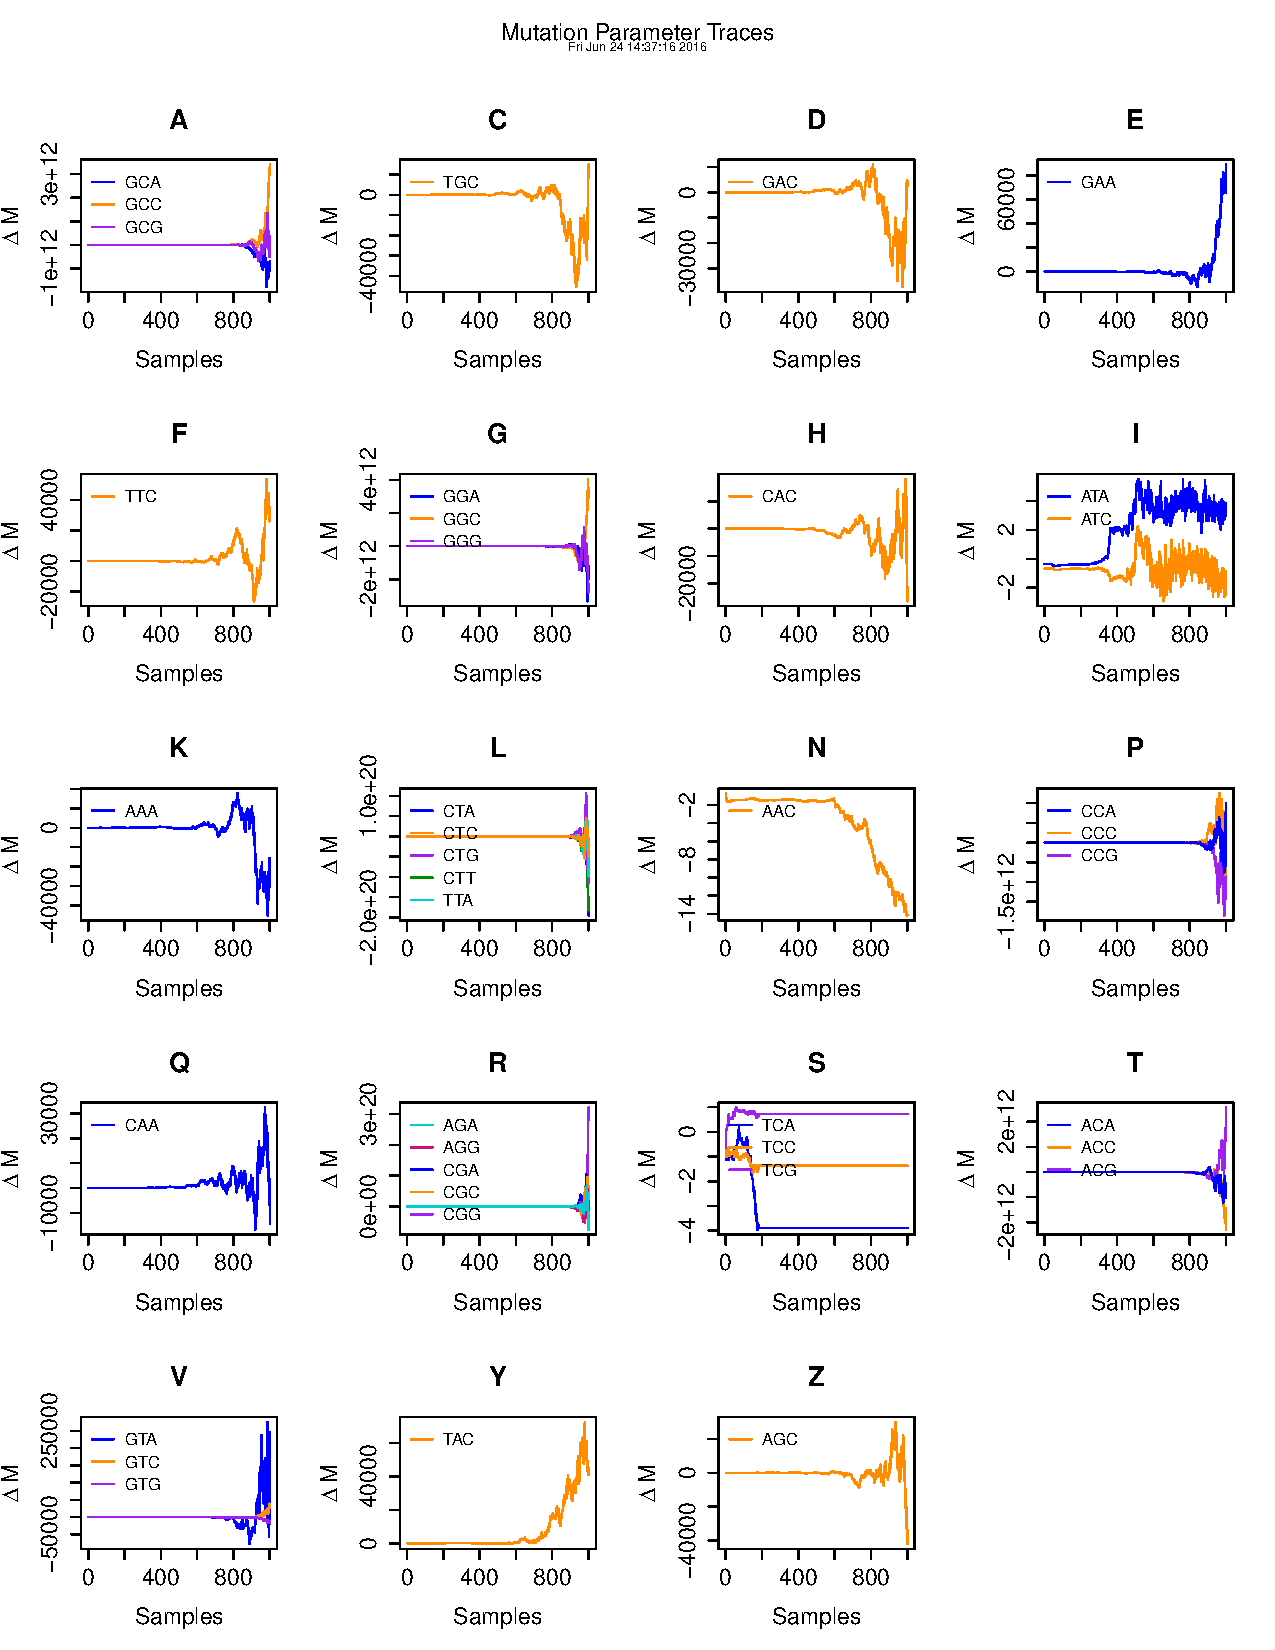
\includegraphics[scale=.65]{FONSE_Plots/June_24/Run2_MutationTrace}
        \caption{Mutation trace for Run 2}
        \label{fig:JUN24_MUT_R2}
    \end{figure}
    \begin{figure}
        \centering
        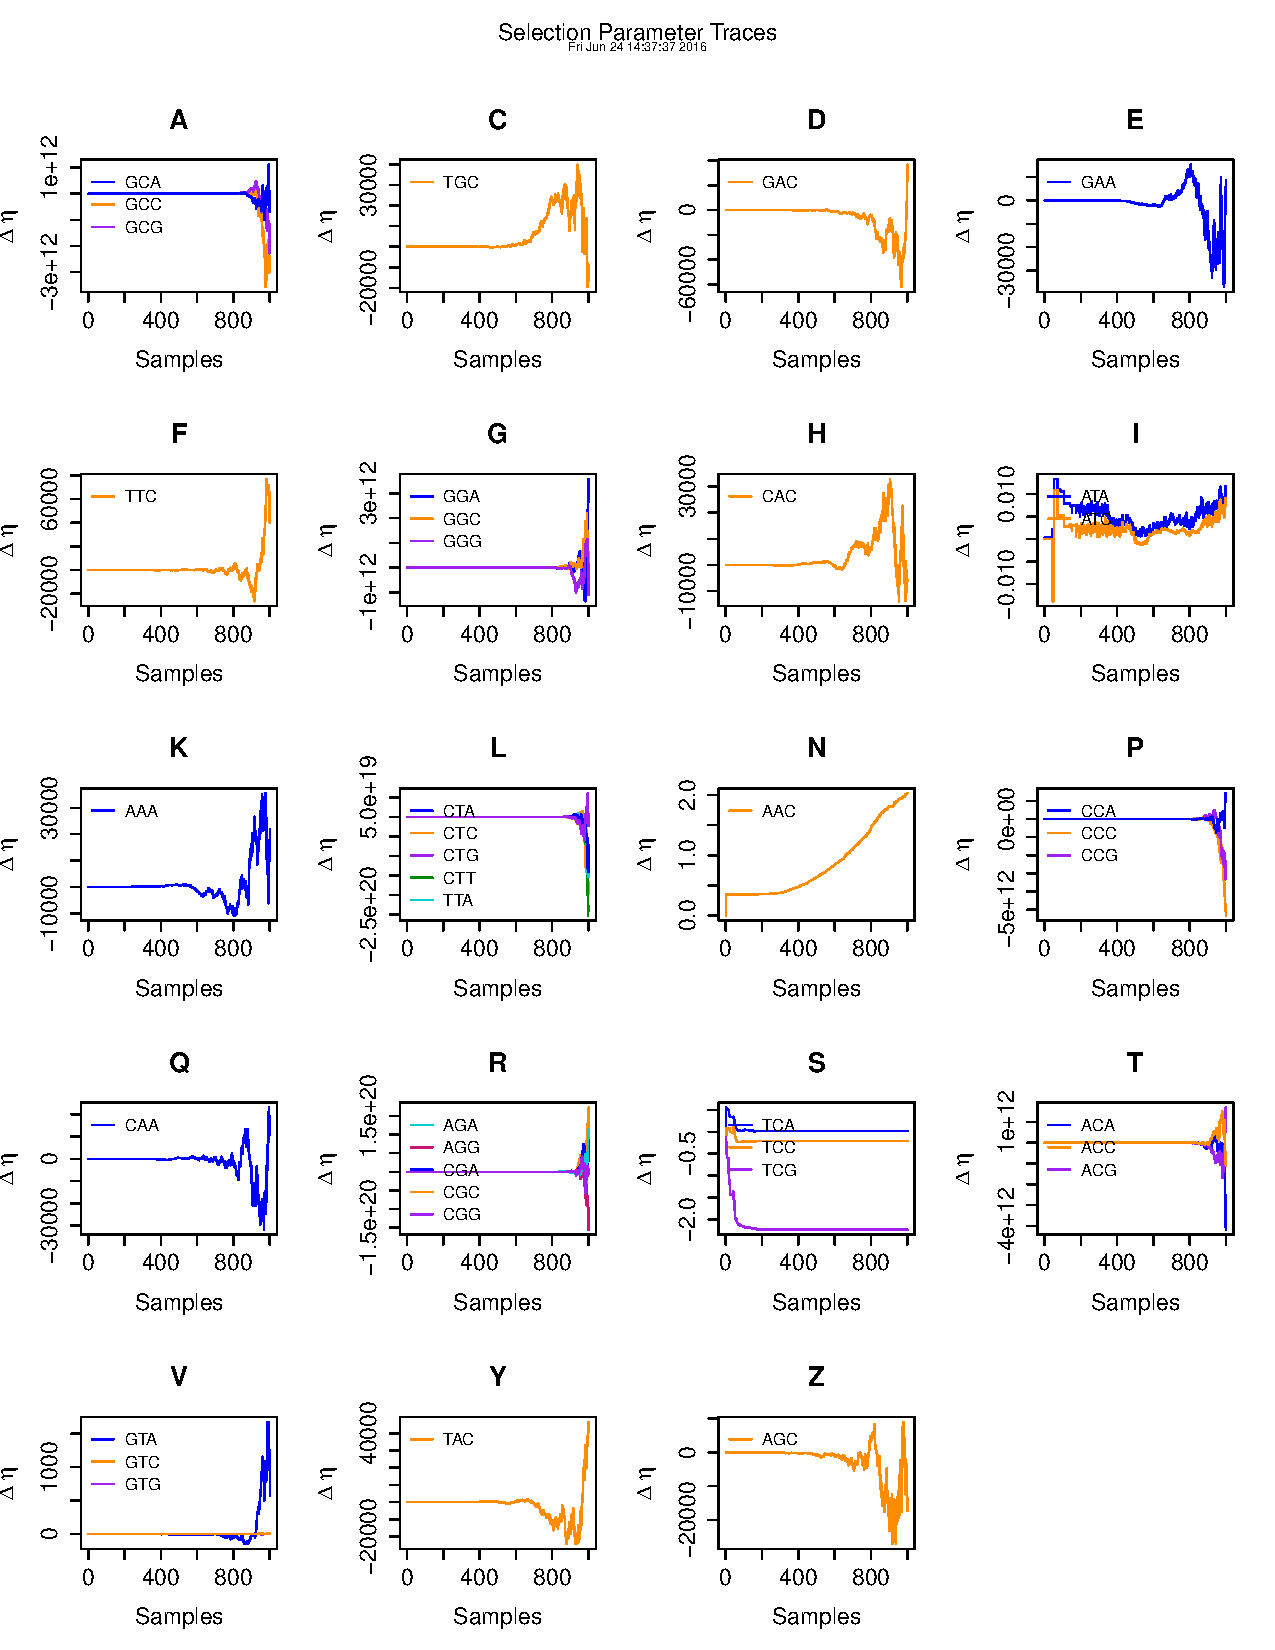
\includegraphics[scale=.65]{FONSE_Plots/June_24/Run2_SelectionTrace}
        \caption{Selection trace for Run 2}
        \label{fig:JUN24_SEL_R2}
    \end{figure}
\end{document}














